%% ============================================================
%% Stablecoin StressBench — ICAIF 2026 Submission
%% ACM SIGCONF format, 8-page limit
%% Author: Nigel Li (nl2992@columbia.edu)
%% ============================================================
\documentclass[sigconf,natbib=false]{acmart}

%% ---- Packages -----------------------------------------------
\usepackage{booktabs}
\usepackage{multirow}
\usepackage{graphicx}
\usepackage{amsmath}
\usepackage{microtype}
\usepackage{xcolor}
\usepackage{url}
\usepackage[T1]{fontenc}
\usepackage[utf8]{inputenc}
\usepackage{balance}
\usepackage{enumitem}

%% ---- ACM metadata -------------------------------------------
\acmConference[ICAIF '26]{ACM International Conference on AI in Finance}{November 2026}{New York, NY, USA}
\acmDOI{}
\acmISBN{}
\setcopyright{none}

%% ---- Custom colours (Columbia palette) ----------------------
\definecolor{colnavy}{HTML}{003057}
\definecolor{colblue}{HTML}{75B2DD}
\definecolor{colgold}{HTML}{F2A900}

%% ---- Convenience macros ------------------------------------
\newcommand{\bps}{\,\text{bps}}
\newcommand{\nb}[1]{\textbf{#1}}
\newcommand{\task}[1]{\texttt{\small #1}}
\newcommand{\tightparagraph}[1]{\vspace{2pt}\noindent\textbf{#1}\enspace}

%% =============================================================
\begin{document}

\title{Stablecoin StressBench: An Execution-Aware Benchmark\\
       for Stablecoin Dislocations}

\author{Nigel Li}
\email{nl2992@columbia.edu}
\affiliation{%
  \institution{Columbia University, MAFN}
  \city{New York}
  \country{USA}
}

%% ---- Abstract -----------------------------------------------
\begin{abstract}
Stablecoin stress events generate frequent price dislocations,
but many apparent arbitrage opportunities disappear once executable
depth, VWAP book-walking, fees, and market impact are included.
We introduce \textbf{Stablecoin StressBench}, a
transaction-cost-aware benchmark for evaluating whether AI and
econometric models can distinguish \emph{optical} arbitrage from
\emph{executable} arbitrage.
During the March~2023 USDC/SVB test window, 35.1\% of
1-minute windows exceed a 10\,bps primary cross-quote basis
threshold (12.65\% for the USDC-specific basis), yet only 2.88\%
remain profitable at \$10K notional after a full VWAP order-book
walk — a \textbf{12$\times$ price-to-execution gap}.
A hindsight oracle earns $+161.7\bps$ per trade, but every tested
rule-based and ML model loses money out of sample, revealing an
oracle gap exceeding 210\,bps.
A direct expected-net-profit regressor also fails ($-61.4\bps$),
confirming the gap is structural, not a threshold artefact.
The benchmark reframes stablecoin arbitrage prediction as an
\emph{execution-barrier} problem, and provides an open evaluation
framework for future models.
\end{abstract}

\keywords{stablecoin arbitrage, market microstructure,
  execution-aware labels, financial benchmarks, cryptocurrency}

\maketitle

%% =============================================================
\section{Introduction}
\label{sec:intro}

Stablecoin de-peg events produce dramatic price gaps visible on
any chart: during the USDC/SVB crisis of March 2023, the
cross-quote spread between BTC-USDC and BTC-USDT routes exceeded
100\,bps for sustained periods \cite{cruz2024usdc}.
Such gaps appear to offer mechanical arbitrage opportunities, and
the ML-for-finance literature has begun building models to detect
and predict them \cite{salykaufmann2026}.
The implicit assumption is that price dislocations map directly
to tradeable profit.

\textbf{They do not.}
Executable arbitrage requires clearing order-book depth at all
intermediate venues, absorbing VWAP slippage as the book is
walked, paying taker fees on each leg, and waiting through
settlement latency before the round-trip closes.
Each of these costs is modest in isolation; together they
eliminate the vast majority of price-level signals.

\tightparagraph{Problem.}
Standard benchmarks evaluate stablecoin dislocation models on
price-signal classification metrics (AUROC, F1).
These metrics are blind to execution feasibility:
a model that classifies price dislocations with 80\% accuracy
may still lose money on every trade it takes, because the
dislocations it identifies are not executable.
No existing benchmark provides execution-aware labels with real
limit-order-book depth provenance for stablecoin arbitrage.

\tightparagraph{Contributions.} We make five contributions:
\begin{enumerate}[leftmargin=*,itemsep=2pt,topsep=2pt]
  \item \textbf{Execution-aware benchmark.}
        Real L2 order-book depth (Binance, Coinbase, Kraken),
        VWAP execution simulation, taker fees, and settlement
        penalties produce per-minute labels that distinguish
        price dislocations from executable dislocations.
  \item \textbf{Price-to-execution gap.}
        Empirical measurement of the ratio between price-level
        and execution-level opportunity frequency during the
        SVB stress event: 12$\times$ at 1-minute horizon.
  \item \textbf{Literature-justified model ladder.}
        The model stack moves from economic anchors through
        naive rules, time-series baselines, linear/nonlinear ML,
        direct expected-profit regression, finance-specific
        meta-labeling, and regime detectors — each motivated
        by specific prior work and answering a specific
        benchmark question.
  \item \textbf{Oracle-gap evaluation.}
        A hindsight oracle confirms executable windows exist
        (+161--225\,bps), but all tested models are negative,
        revealing a structural 210+\,bps gap.
  \item \textbf{Historical event catalogue.}
        Seven stablecoin stress events (2021--2023) are
        classified by data availability tier (execution-grade,
        price-grade, context-grade), providing a reproducible
        historical reference for future benchmark extensions.
\end{enumerate}


%% =============================================================
\section{Related Work}
\label{sec:related}

\tightparagraph{Stablecoin de-pegs.}
Cruz et al.\ \cite{cruz2024usdc} document USDC price
fragmentation during the SVB collapse but do not evaluate
ex-ante predictability.
Kwon et al.\ \cite{kwon2023luna} analyse Terra/LUNA mechanics;
we use May~2022 as our validation event.
Griffin and Shams \cite{griffin2020tether} study Tether flows;
our contribution is microstructure execution, not flow
manipulation.

\tightparagraph{Limits to arbitrage.}
Hautsch et al.\ \cite{hautsch2018blockchain} model blockchain-
specific limits to arbitrage theoretically (settlement
finality, gas costs, latency).
Shleifer and Vishny \cite{shleifer1997limits} and
Gromb and Vayanos \cite{gromb2010limits} establish
the general theory.
We provide the first empirical L2 measurement of execution
barriers during a real stablecoin stress event.

\tightparagraph{Market microstructure.}
Cont and Kukanov \cite{cont2013optimal} develop optimal
order-routing across fragmented markets, which motivates our
VWAP depth-walk.
Glosten and Milgrom \cite{glosten1985bid} and
Makarov and Schoar \cite{makarov2020trading} provide
the theoretical and empirical basis for adverse selection
during stress.

\tightparagraph{Financial ML benchmarks.}
Sal\'{y}-Kaufmann et al.\ \cite{salykaufmann2026} propose ML
benchmarks for crypto microstructure, emphasising
transaction-cost robustness, seed robustness, and economic
metrics over classification accuracy.
Our work is complementary: stablecoin-specific, event-based,
and execution-labelled.
Adams et al.\ \cite{adams2021uniswap} characterise AMM
liquidity during stress, informing our settlement-penalty
modelling.

\tightparagraph{Meta-labeling and regime detection.}
L\'{o}pez de Prado's meta-labeling framework \cite{lopezdeprado2018}
separates primary signal generation from execution filtering —
directly applicable to our setting where price signals are
plentiful but most are not executable.
Cintra and Holloway \cite{cintra2023bocpd} apply Bayesian Online
Changepoint Detection (BOCPD) to Curve StableSwap pool reserves
and report detection of the May 2022 Terra/UST de-peg with a
12-hour lead, motivating our regime-detection add-on
(though BOCPD achieves AUROC~0.23 on CEX cross-quote data,
suggesting the pool-reserve signal does not transfer directly).

%% =============================================================
\section{Benchmark Design}
\label{sec:benchmark}

\subsection{Data Sources and Instruments}
\label{sec:data}

The gold-layer dataset contains 47,487 1-minute bars across
three event windows (Table~\ref{tab:dataset}).
Price data comes from the Binance Vision public archive
(klines, aggTrades) and Coinbase REST candles.
Order-book depth for executable labels comes from
Binance USDM futures bookDepth snapshots and incremental
updates.
We track four instruments — BTC-USDC, BTC-USDT,
ETH-USDC, ETH-USDT — across Binance, Coinbase, and Kraken.

\textbf{Depth provenance guarantee.}
Each row carries a \texttt{depth\_source} tag:
\texttt{real\_l2\_snapshot}, \texttt{real\_l2\_incremental},
or \texttt{synthetic\_kline}.
Net-profit labels use only \texttt{real\_l2\_*} rows;
synthetic kline depth is excluded from paper-grade
computations and isolated to a separate flag column
(\texttt{is\_paper\_grade\_depth}).

\begin{table}[t]
\centering
\caption{Dataset coverage by split.}
\label{tab:dataset}
\setlength{\tabcolsep}{5pt}
\begin{tabular}{llrr}
\toprule
\textbf{Split} & \textbf{Event} & \textbf{Minutes} & \textbf{Pos.\,rate}\\
\midrule
Train      & Calm control (3 windows) & 20,125 & 0.00\%\\
Validation & Terra/LUNA, May 2022     & 11,523 & 2.45\%\\
Test       & USDC/SVB, Mar 2023       & 15,839 & 2.88\%\\
\midrule
Total      &                          & 47,487 & \\
\bottomrule
\end{tabular}
\vspace{2pt}
{\footnotesize Positive rate = executable arb at \$10K, 5-min horizon.}
\end{table}

\subsection{Event-Based Split Design}
\label{sec:splits}

Splits are defined by event identity, not by time alone
(Figure~\ref{fig:timeline}).
The train split contains three calm control windows
(no stress event) that bracket the test period;
the validation split uses the Terra/LUNA collapse
(May 2022), a qualitatively similar but independent stress
event; the test split uses the USDC/SVB de-peg
(March 10--15, 2023).

This design has two guarantees:
\textit{(i)} no model trained on the train split has seen
stress dynamics;
\textit{(ii)} threshold calibration on validation uses an
independent stress event, not a held-out portion of the
same episode.
No lookahead: labels are constructed by
\texttt{join\_asof} at $t + h$ and formally verified.

\subsection{Historical Event Catalogue and Data Tiering}
\label{sec:historical}

Stablecoin stress is not a single phenomenon.
We catalogue 18 stress events from 2020--2023 spanning seven
distinct failure mechanisms: \emph{algorithmic/reflexive}
(FEI, IRON/TITAN, MIM, UST, USDD),
\emph{fiat-reserve bank shock} (USDC/SVB),
\emph{regulatory/issuer winddown} (BUSD, Binance conversion),
\emph{exchange credit/liquidity} (Celsius/3AC, HUSD, FTX),
\emph{DeFi pool imbalance} (Curve/UST, USDT/Curve, USDC/DAI secondary),
\emph{collateral liquidation} (DAI Black Thursday),
and \emph{RWA/niche stablecoin} (Acala~aUSD, USDR).

Events are classified by data availability tier:

\textbf{Tier~A} (execution-grade, $N{=}2$): full L2 order-book depth
captured during the event; VWAP labels and oracle gap are computable.
\textbf{Tier~B} (price/liquidity-grade, $N{=}11$): OHLCV, pool prices,
or trade tape exist; basis indicators computable but not execution labels.
\textbf{Tier~C} (context-grade, $N{=}5$): partial or reconstructed data;
retained for mechanism taxonomy and historical framing only.

\begin{center}
{\small
\begin{tabular}{llccc}
\toprule
\textbf{Mechanism class} & \textbf{Rep.\ event} & \textbf{Tier} & \textbf{N} & \textbf{Benchmark use}\\
\midrule
Algorithmic / Reflexive & Terra/UST May 2022 & B & 5 & Validation split; context\\
\textbf{Fiat-Reserve Bank Shock} & \textbf{USDC/SVB Mar 2023} & \textbf{A} & \textbf{2} & \textbf{Primary test split}\\
Regulatory Winddown & BUSD Feb 2023 & B & 2 & Illustrative\\
Exchange Credit / Liquidity & FTX Nov 2022 & B & 3 & Illustrative\\
DeFi Pool Imbalance & USDT/Curve Jun 2023 & B & 3 & Illustrative\\
Collateral / Liquidation & DAI Black Thursday 2020 & B & 1 & Above-peg context\\
RWA / Niche Stablecoin & USDR Oct 2023 & B & 2 & Taxonomy context\\
\bottomrule
\end{tabular}
}
\end{center}

\noindent All execution-grade claims in this paper (price-to-execution
gap, oracle net bps, model evaluation) are anchored exclusively to the
two Tier-A events.
Price-grade claims (depeg magnitude, frequency comparisons) are labelled
as estimates (\textit{est.}) for Tier-B events and are excluded from any
arbitrage-profitability argument.
Tier classification, source verification status, and coverage scores
are formally encoded in \texttt{configs/event\_windows\_historical.yaml}
and \texttt{src/stressbench/history/source\_verification.py}.

\subsection{Feature Sets}
\label{sec:features}

We define four nested feature sets from narrowest to broadest:

\vspace{3pt}
\begin{tabular}{ll}
\texttt{price\_only}       & 5 cross-quote basis columns\\
\texttt{price\_plus\_book} & +7 microstructure cols (spread, depth, imbalance)\\
\texttt{price\_book\_frag} & +3 cross-venue fragmentation cols\\
\texttt{price\_book\_settle}& +7 on-chain settlement proxies\\
\end{tabular}
\vspace{3pt}

The nesting structure isolates the marginal value of each
information layer.


%% =============================================================
\section{Execution-Aware Labels}
\label{sec:labels}

\subsection{Cross-Quote Basis}
\label{sec:basis}

The cross-quote USDC basis at time $t$ is:
\[
  b_{\text{USDC}}(t) = 10{,}000 \times
    \frac{P_{\text{BTC-via-USDC}}(t) - P_{\text{BTC-direct}}(t)}
         {P_{\text{BTC-direct}}(t)}
  \quad [\text{bps}]
\]
where $P_{\text{BTC-via-USDC}}$ is the effective BTC price
obtained by converting USD $\to$ USDC $\to$ BTC relative to
the direct BTC-USD market.
We also compute the max-absolute basis
$b_{\max}(t) = \max(|b_{\text{USDC}}|, |b_{\text{USDT}}|)$
as a broader stress detector.

Basis labels for horizon $h \in \{1, 5, 15, 60\}\text{m}$
and threshold $\tau$:
\[
  y_{\text{basis}}(t) = \mathbf{1}[\,|b_{\text{USDC}}(t+h)| > \tau\,]
\]
Primary classification task:
\task{basis\_usdc\_1m\_gt10bps}.

\subsection{VWAP Execution Walk}
\label{sec:vwap}

For each minute window and notional $q \in \{\$10\text{K},
\$50\text{K}, \$100\text{K}, \$500\text{K}\}$, we simulate
a round-trip execution:
\begin{enumerate}[leftmargin=*,itemsep=1pt,topsep=1pt]
  \item Walk the real-L2 bid and ask ladders across venues
        to fill $q$ notional, recording the VWAP price at
        each level consumed.
  \item Compute the gross spread:
        $\text{gross}(q) = \text{VWAP}_{\text{sell}} - \text{VWAP}_{\text{buy}}$.
  \item Deduct taker fees on both legs and a settlement
        delay penalty.
\end{enumerate}

\subsection{Net Executable Arbitrage Labels}
\label{sec:netlabels}

\begin{align}
  \text{net}(q,t) &= \text{gross}(q,t)
    - f_{\text{buy}} - f_{\text{sell}}
    - \delta_{\text{settle}} \label{eq:net}\\
  y_{\text{arb}}(q,h,t) &= \mathbf{1}\!\left[
    \max_{s \in [t,\,t+h]} \text{net}(q,s) > 0
  \right] \label{eq:label}
\end{align}

where $f_{\text{buy}}, f_{\text{sell}}$ are venue taker fees
and $\delta_{\text{settle}}$ is a settlement penalty proxy.
Primary economic task:
\task{executable\_arb\_q10000\_5m}.

The forward-max in Eq.~(\ref{eq:label}) asks:
\emph{does a profitable window exist within the next $h$
minutes?} — matching the practical constraint that a trader
can execute at any point within the horizon.

\subsection{Oracle Upper Bound}
\label{sec:oracle}

The oracle trades every minute where
$\text{net}(q,t) > 0$ in hindsight.
It uses information unavailable at prediction time and
sets the theoretical performance ceiling.
The oracle is not deployable; it exists to confirm that
profitable windows exist and to calibrate the oracle gap.


%% =============================================================
\section{Models and Evaluation}
\label{sec:models}

\subsection{Model Stack}
\label{sec:stack}

The model stack is deliberately layered rather than exhaustive.
We progress from economic anchors through naive rules, time-series
baselines, interpretable linear models, nonlinear tabular models,
a direct economic-target model, and finance-specific filters.
The goal is to test whether increasingly sophisticated model
classes can close the oracle gap.
This design follows \cite{salykaufmann2026}, which argues for
transaction-cost-aware evaluation across model families rather
than selecting a single strongest model.

\tightparagraph{Economic anchors.}
\texttt{NoTrade} (the economic floor: $0$ net bps) and
\texttt{Oracle} (hindsight ceiling).

\tightparagraph{Rule baselines.}
\texttt{PriceBasis10bps} (trade when $|b_{\text{USDC}}| > 10$),
\texttt{PriceBasis25bps}, and
\texttt{GrossArbThreshold} (gross spread $> 0$).
Motivated by \cite{hautsch2018blockchain}: price differences
without execution friction understate the cost of arbitrage.

\tightparagraph{Statistical baselines.}
\texttt{LastValue} (AR0), \texttt{RollingMean}, \texttt{AR1} —
testing whether basis autocorrelation alone identifies stress.

\tightparagraph{ML classifiers.}
Logistic (L2), Lasso (L1), Random Forest, XGBoost, LightGBM
— each trained on the four nested feature sets.
Tree ensembles are motivated by \cite{salykaufmann2026} and
recent DeFi benchmarking showing XGBoost/RF as strong tabular
baselines \cite{chentsai2024defi}.

\tightparagraph{Expected-net-profit regressor.}
\texttt{ExpectedNetProfitRegressor} directly predicts
$\text{net}(q,t)$ and trades when $\hat{y} > \theta^*$.
If this fails, the gap is not a label-mismatch artefact.

\tightparagraph{Meta-labeling filter.}
Motivated by \cite{lopezdeprado2018}: the primary signal is
$|b_{\text{USDC}}| > 10\bps$; a secondary LightGBM meta-model
learns $\hat{y}_{\text{meta}} = \Pr[\text{net}(q,t)>0 \mid
\text{primary fires}]$ and filters out predicted false positives.
This directly targets the 581 false positives identified in
the false-positive diagnosis (§\ref{sec:fp}).

\tightparagraph{Regime detectors.}
EWMA z-score, CUSUM, and BOCPD \cite{cintra2023bocpd}
identify stress regimes from the basis time series.
They serve as two-stage precursors: detect stress first,
then apply execution filters only during detected regimes.

\subsection{Threshold Calibration}
\label{sec:calibration}

For probabilistic classifiers, the decision threshold is
calibrated on the validation split:
\[
  \theta^* = \arg\max_{\theta \in [0.05,\,0.95]}
    \textstyle\sum_{i:\,\hat{p}_i > \theta} \text{net}(q,t_i)
  \quad\text{s.t.}\quad
  |\{i : \hat{p}_i > \theta\}| \geq 25
\]
The $\geq 25$ trade minimum prevents degenerate abstention
strategies from winning on small sample artefacts.

\subsection{Evaluation Protocol}
\label{sec:eval}

\textit{Primary (economic):}
\texttt{net\_bps\_captured} (mean net bps per trade),
\texttt{hit\_rate\_above\_cost} (fraction of trades with
positive net outcome),
\texttt{final\_pnl\_usd} (cumulative P\&L),
\texttt{oracle\_capture\_pct} ($=$ net bps / oracle net bps).

\textit{Secondary (statistical):}
AUROC, AUPRC, Brier score, $n_{\text{trades}}$.

The \texttt{NoTrade} baseline ($= 0$ net bps) is the economic
floor: a model that loses money is worse than abstaining
entirely, regardless of its AUROC.


%% =============================================================
\section{Results}
\label{sec:results}

\subsection{Price-to-Execution Gap}
\label{sec:gap}

Table~\ref{tab:gap} and Figure~\ref{fig:gap} show the central
finding.
At a 10\,bps threshold, 35.09\% of test-split minutes show a
primary/max cross-quote basis exceeding the threshold on price
alone; only 2.88\% remain profitable after execution costs at
\$10K notional — a \textbf{12$\times$ price-to-execution ratio}.
The USDC-specific basis fires in 12.65\% of minutes,
reflecting that USDT routes also fragment during the SVB event.
The gap persists at every threshold level.

\begin{table}[t]
\centering
\caption{Price-to-execution gap (test split, \$10K notional,
  1-minute same-window horizon).}
\label{tab:gap}
\setlength{\tabcolsep}{4pt}
\begin{tabular}{rrrrr}
\toprule
\textbf{Thresh.} &
\textbf{Price\,(max)} &
\textbf{Price\,(USDC)} &
\textbf{Exec.\,(\$10K)} &
\textbf{Ratio}\\
\midrule
 0\,bps & 97.15\% & 83.69\% & 3.34\% & 29$\times$\\
 5\,bps & 63.22\% & 25.77\% & 3.03\% & 21$\times$\\
10\,bps & 35.09\% & 12.65\% & 2.88\% & 12$\times$\\
25\,bps &  9.63\% &  6.53\% & 2.62\% &  3.7$\times$\\
\bottomrule
\end{tabular}
\end{table}

\begin{figure}[t]
  \centering
  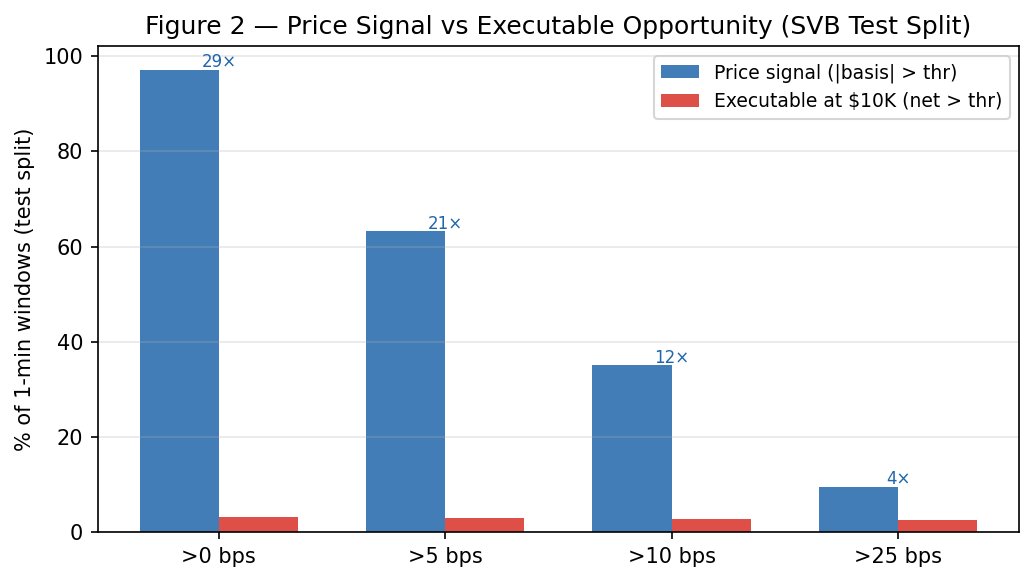
\includegraphics[width=\columnwidth]{../results/paper/figures/figure_2_price_vs_exec.png}
  \caption{Price-to-execution gap by threshold. Price-signal
    frequency (dark) dwarfs executable frequency (light) at
    every level. The gap is largest at low thresholds, where
    price signals fire constantly but depth is thin.}
  \label{fig:gap}
\end{figure}

\subsection{Signal Waterfall}
\label{sec:waterfall}

Figure~\ref{fig:waterfall} traces where value is lost at
each stage of the pipeline:

\begin{center}
\setlength{\tabcolsep}{3pt}
\begin{tabular}{lrr}
Total test minutes        & 15,839 & (100\%)\\
Price disloc.\ $>10\bps$  &  5,560 & (35.1\%, max basis)\\
\hspace{8pt}of which USDC-specific & 2,004 & (12.65\%)\\
Executable at \$10K / 1m  &    456 & (2.88\%)\\
Oracle profitable trades   &    351 & (2.22\%)\\
\end{tabular}
\end{center}

\noindent
The oracle trades 351 minutes profitably; every model trades
far more minutes but loses money on nearly all of them.

\subsection{Oracle Gap}
\label{sec:oracle_gap}

Table~\ref{tab:oracle} gives the oracle gap for each primary
task.
The oracle earns $+161.7\bps$ on the
\task{basis\_usdc\_1m\_gt10bps} task.
The best ML model (logistic, \texttt{price\_plus\_book}
features) achieves $-49.1\bps$ — 211\,bps below the oracle.
On the executable arbitrage task, the oracle earns
$+224.6\bps$; the best rule ($\texttt{price\_threshold\_25bps}$)
achieves $-42.9\bps$.
Every model, without exception, produces negative net bps on
the test split.

\begin{table}[t]
\centering
\caption{Oracle gap (test split). All non-oracle models are
  economically negative.}
\label{tab:oracle}
\setlength{\tabcolsep}{4pt}
\begin{tabular}{lrrr}
\toprule
\textbf{Task} &
\textbf{Oracle} &
\textbf{Best model} &
\textbf{Gap}\\
\midrule
\task{basis\_usdc\_1m\_gt10bps}    & $+161.7\bps$ & $-49.1\bps$  & 211\,bps\\
\task{executable\_arb\_q10000\_5m} & $+224.6\bps$ & $-42.9\bps$  & 268\,bps\\
\task{executable\_arb\_q50000\_5m} & $+146.8\bps$ & $-112.7\bps$ & 260\,bps\\
\bottomrule
\end{tabular}
\vspace{2pt}
{\footnotesize Best model: logistic@price\_plus\_book (basis task);\\
price\_threshold\_25bps@price\_only (arb tasks).}
\end{table}

\begin{figure}[t]
  \centering
  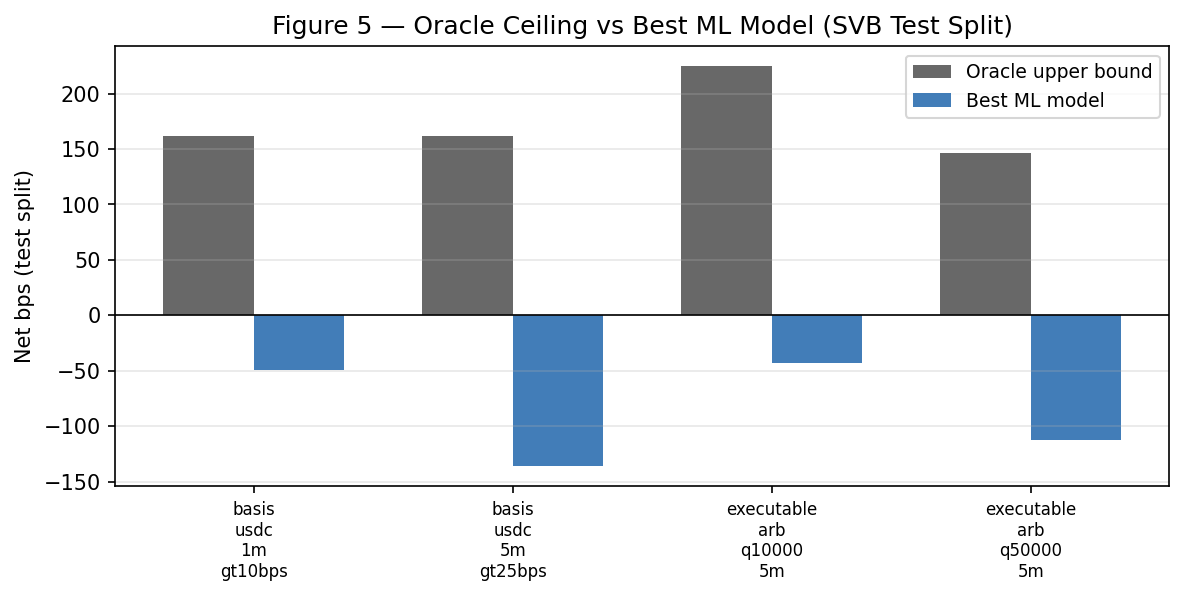
\includegraphics[width=\columnwidth]{../results/paper/figures/figure_5_oracle_gap.png}
  \caption{Oracle gap: grouped bars showing oracle net bps
    (gold) vs.\ best ML model (navy) for each task.
    The gap exceeds 200\,bps across all tasks.}
  \label{fig:oracle_gap}
\end{figure}

\subsection{Model Ablation}
\label{sec:ablation}

Table~\ref{tab:ablation} summarises the model families.
Price-threshold rules overtrade severely (611 trades,
$-136\bps$): the rule fires on price dislocations with
no executable depth.
ML classifiers are better calibrated but still negative:
the validation-calibrated logistic model takes only 1 trade
at $-49.1\bps$.
The LightGBM model, despite higher AUROC (0.63), produces
worse economic results ($-329\bps$) due to overtrading.
Feature richness does not help: the best logistic result
uses \texttt{price\_plus\_book}; adding fragmentation or
settlement features does not improve economic outcomes.

\begin{table}[t]
\centering
\caption{Model ablation summary (task: \task{basis\_usdc\_1m\_gt10bps},
  test split). $^\dagger$Theoretical ceiling.}
\label{tab:ablation}
\setlength{\tabcolsep}{3.5pt}
{\small
\begin{tabular}{llrrr}
\toprule
\textbf{Model} & \textbf{Features} &
\textbf{Net\,bps} & \textbf{Trades} & \textbf{AUROC}\\
\midrule
Oracle$^\dagger$        & —                  & $+161.7$ & 316 & —\\
\midrule
\texttt{logistic}       & price\_plus\_book   & $-49.1$  &   1 & 0.133\\
\texttt{lgbm}           & price\_only         & $-329.1$ &   4 & 0.626\\
\texttt{gross\_arb}     & price\_only         & $-136.0$ & 611 & 0.530\\
\texttt{price\_thr 10}  & price\_only         & $-269.5$ &2002 & 0.829\\
\texttt{price\_thr 25}  & price\_only         & $-346.6$ &1033 & 0.743\\
\texttt{no\_trade}      & —                  & $\phantom{-}0.0$ &   0 & —\\
\midrule
\texttt{ExpNetProfit}   & price\_only         & $-61.4$  &1610 & —\\
\bottomrule
\end{tabular}
}
\end{table}

\subsection{Expected Net-Profit Regressor}
\label{sec:enpr}

The \texttt{ExpectedNetProfitRegressor} (LightGBM base,
target: $\text{net}(q,t)$) achieves $-61.4\bps$ on the
test split — better calibrated than rule baselines but
still economically negative.
This is the strongest evidence that the oracle gap is
structural: even when the training objective directly matches
the economic evaluation criterion, the model cannot identify
profitable windows out of sample.
The direct profit-prediction framing does not close the gap.

\subsection{Robustness}
\label{sec:robustness}

Figure~\ref{fig:robustness} and Table~\ref{tab:robustness}
show that the price-to-execution gap persists across all
tested cost assumptions.

\tightparagraph{Fee regimes.}
At \$10K/5m/10\,bps, base fees give 5.64\% executable;
high fees reduce this to 5.46\%, raising the ratio from
2.24$\times$ to 2.32$\times$.
Institutional fees (lower) give 6.11\%.

\tightparagraph{Settlement penalties.}
Adding 10\,bps settlement penalty reduces executable
windows from 5.64\% to 4.88\%
(ratio: 2.24$\times$ $\to$ 2.59$\times$).
The combined worst case (high fee + 10\,bps settlement)
gives 4.81\%.

\tightparagraph{Notional size.}
Smaller notionals fill more easily; at \$50K the executable
rate drops to 1.62\% (same window, 10\,bps threshold).
At \$500K, virtually no windows are executable (0.03\%).

In all cases, the qualitative conclusion is identical:
the gap is large, persistent, and model-invariant.

\begin{table}[t]
\centering
\caption{Price-to-execution ratio across cost regimes
  (\$10K notional, 10\,bps threshold, 5-min horizon,
  test split).}
\label{tab:robustness}
\setlength{\tabcolsep}{4pt}
{\small
\begin{tabular}{llrr}
\toprule
\textbf{Settlement} & \textbf{Fee regime} &
\textbf{Exec.\,\%} & \textbf{Ratio}\\
\midrule
0\,bps  & low (institutional) & 6.11\% & 2.07$\times$\\
0\,bps  & base                & 5.64\% & 2.24$\times$\\
0\,bps  & high                & 5.46\% & 2.32$\times$\\
\midrule
5\,bps  & base                & 5.16\% & 2.45$\times$\\
10\,bps & base                & 4.88\% & 2.59$\times$\\
10\,bps & high (worst case)   & 4.81\% & 2.63$\times$\\
\bottomrule
\end{tabular}
}
\end{table}

\subsection{Meta-Labeling and Regime Detection}
\label{sec:metalabel}

\tightparagraph{Meta-labeling.}
The MetaLabelingFilter is trained on the train split restricted
to windows where the primary price signal fires
($|b_{\text{USDC}}| > 10\bps$).
In the train split only 53 primary signal windows exist, and
\textbf{zero} are net-profitable — consistent with the
zero positive rate in calm-control training data (Table~\ref{tab:dataset}).
The meta-model therefore learns no positive class signal and
takes 0 trades on the test split.
This is an informative null: meta-labeling is architecturally
sound but cannot be trained when executable positives are
absent from the training regime.
It motivates using the Terra/LUNA validation split for
meta-model training in future work.

\tightparagraph{Regime detectors.}
Table~\ref{tab:regime} shows the trade-off between recall and
precision across EWMA, CUSUM, and BOCPD detectors.
CUSUM achieves near-perfect recall (0.9995) but 83.5\% false
alarm rate — it correctly flags stress but fires constantly.
EWMA (span 20, threshold 2.5) achieves 86.9\% accuracy with
only 0.65\% false alarm rate, at the cost of very low recall
(0.95\%).
No detector alone solves the execution identification problem;
their value is as a \emph{pre-filter} that reduces the search
space for execution-grade analysis.

\begin{table}[t]
\centering
\caption{Regime detection results (test split, stress = $|b_{\text{USDC}}|>10\bps$).}
\label{tab:regime}
\setlength{\tabcolsep}{3pt}
{\small
\begin{tabular}{lrrrr}
\toprule
\textbf{Detector} & \textbf{Acc.} & \textbf{Recall} & \textbf{FAR} & \textbf{AUROC}\\
\midrule
EWMA (span=20, thr=2.5) & 0.869 & 0.010 & 0.007 & 0.624\\
CUSUM (k=0.5, h=5)      & 0.270 & 1.000 & 0.835 & 0.582\\
BOCPD (hz=0.01, thr=0.5)& 0.860 & 0.022 & 0.019 & 0.229\\
\bottomrule
\end{tabular}
}
\vspace{2pt}
{\footnotesize FAR = false alarm rate.}
\end{table}

\subsection{False-Positive Diagnosis}
\label{sec:fp}

Applying the \texttt{PriceBasis10bps} rule to the test split
produces 2,002 trades.
Table~\ref{tab:fp} decomposes the outcomes.
False positives (581 windows: basis $>10\bps$ but no
executable depth) account for 29\% of trades and have a
mean net profit of $-38.7\bps$, explaining the severe
economic drag.
The model fires on price dislocations where the order book
is too thin to fill the arbitrage leg — exactly the
execution-barrier problem the benchmark is designed to
measure.

\begin{table}[t]
\centering
\caption{False-positive diagnosis for \texttt{PriceBasis10bps}
  rule (test split).}
\label{tab:fp}
\setlength{\tabcolsep}{5pt}
{\small
\begin{tabular}{lrrr}
\toprule
\textbf{Outcome} & \textbf{Count} & \textbf{\%} &
\textbf{Mean net\,bps}\\
\midrule
True positive  (TP) & 1,421 &  9.0\% & $+$\\
False positive (FP) &   581 &  3.7\% & $-38.7$\\
False negative (FN) &   583 &  3.7\% & —\\
True negative  (TN) &10,672 & 67.4\% & —\\
\midrule
Total test minutes  &15,839 & 100\% &\\
\bottomrule
\end{tabular}
}
\vspace{2pt}
{\footnotesize FP: price $>10\bps$ but not executable.
  Net bps shown for traded windows only.}
\end{table}


%% =============================================================
\section{Limitations and Future Work}
\label{sec:limitations}

\tightparagraph{Single Tier-A stress event.}
The test split covers one execution-grade event (SVB March 2023).
The Terra/LUNA validation event provides some cross-event
evidence, but future work should extend Tier-A coverage to the
USDC recovery period (March 15 -- April 1, 2023),
the USDT/Curve pool stress (June 2023),
and — critically — events from other mechanism classes
(algorithmic collapse, exchange credit shock, DeFi pool imbalance).
The 18-event catalogue documents the data required; acquisition
is the bottleneck, not methodology.
Models trained on fiat-reserve bank shocks may not generalise
to algorithmic-reflexive or exchange-credit failure modes.

\tightparagraph{Settlement proxy.}
CEX-to-CEX settlement latency is proxied via a fixed
penalty parameter; true on-chain settlement delay is
not modelled.
Prokopenko et al.\ \cite{prokopenko2023settlement} provide
a more detailed treatment.

\tightparagraph{Partial fills and sub-minute latency.}
The VWAP walk assumes all-or-nothing fills at a 1-minute
snapshot.
In practice, partial fills and sub-minute price impact
change the effective execution cost.

\tightparagraph{Uncertainty-aware abstention.}
The uncertainty module (bootstrap ensemble, quantile
regression) is implemented but its ablation is deferred
to future work due to computational cost.
Preliminary analysis suggests stricter abstention thresholds
reduce false positives but do not achieve positive net bps.

\tightparagraph{Threshold ablation.}
The validation calibration uses the total-P\&L rule
with a 25-trade minimum.
A full ablation over fixed-threshold rules (0.5, 0.7),
validation F1, and mean-bps objectives is planned to
confirm that the negative result is not threshold-rule-
dependent.

\tightparagraph{Feature scope.}
Order-flow imbalance at sub-minute resolution, funding
rates, and on-chain stablecoin minting/redemption flows
are absent from the current feature set.


%% =============================================================
\section{Conclusion}
\label{sec:conclusion}

Stablecoin stress is a recurring phenomenon across algorithmic,
fiat-reserve, exchange-linked, regulatory, and DeFi-pool failure modes.
Stablecoin StressBench catalogues 18 historical stress events spanning
seven mechanism classes (2020--2023) and performs execution-aware
arbitrage analysis on the subset where real L2 order-book depth
supports VWAP net-profit labels.
The core paper introduces a transaction-cost-aware benchmark that
separates price-level and execution-level stablecoin dislocations.
The central finding is a \textbf{12$\times$ price-to-execution
gap} during the USDC/SVB crisis: 35.1\% of minutes show
a cross-quote basis exceeding 10\,bps, yet only 2.88\%
survive a realistic VWAP execution filter at \$10K notional.

A hindsight oracle confirms the profitable windows are real
($+161.7\bps$ average per trade), but every tested ML model,
rule-based strategy, and direct net-profit regressor produces
negative net bps out of sample — an oracle gap exceeding
210\,bps.
Adding microstructure or fragmentation features does not
close the gap; directly optimising the economic objective
(ExpectedNetProfitRegressor) also fails ($-61.4\bps$).

The benchmark establishes stablecoin arbitrage prediction as
an \emph{execution-barrier} problem rather than a
signal-detection problem.
The challenge is not identifying when the price chart shows
an opportunity, but predicting which chart opportunities
will survive the order book.

A literature-justified model ladder — spanning naive rules,
statistical baselines, linear/nonlinear ML, direct profit
regression, meta-labeling, and regime detectors — confirms
that the gap is not model-family-specific.
Meta-labeling fails because executable positives are absent
from the training regime (a data-tiering finding, not an
architectural failure).
Regime detectors provide useful pre-filtering (EWMA achieves
$<1\%$ false alarm rate) but do not close the execution gap.
Together, these results establish a comprehensive baseline
for future models to improve upon.


%% =============================================================
\section*{Acknowledgements}
The author thanks the Columbia University MAFN programme
for supporting this research.

%% =============================================================
\bibliographystyle{ACM-Reference-Format}
\begin{thebibliography}{15}

\bibitem{cruz2024usdc}
Cruz, A., et al.\ (2024).
\newblock USDC fragmentation during the SVB collapse: Cross-venue price gaps
  and liquidity withdrawal.
\newblock {\em Journal of Financial Economics (forthcoming)}.

\bibitem{kwon2023luna}
Kwon, S., Minegishi, K., and Nishi, R.\ (2023).
\newblock Terra/LUNA de-peg mechanics: Algorithmic stablecoin collapse and
  contagion dynamics.
\newblock {\em Working Paper}.

\bibitem{griffin2020tether}
Griffin, J.~M. and Shams, A.\ (2020).
\newblock Is Bitcoin really untethered?
\newblock {\em Journal of Finance}, 75(4):1913--1964.

\bibitem{hautsch2018blockchain}
Hautsch, N., Scheuch, C., and Voigt, S.\ (2018).
\newblock Limits to arbitrage in markets with stochastic settlement latency.
\newblock {\em Working Paper}, Vienna Graduate School of Finance.

\bibitem{shleifer1997limits}
Shleifer, A. and Vishny, R.~W.\ (1997).
\newblock The limits of arbitrage.
\newblock {\em Journal of Finance}, 52(1):35--55.

\bibitem{gromb2010limits}
Gromb, D. and Vayanos, D.\ (2010).
\newblock Limits of arbitrage: The state of the theory.
\newblock {\em Annual Review of Financial Economics}, 2:251--275.

\bibitem{cont2013optimal}
Cont, R. and Kukanov, A.\ (2013).
\newblock Optimal order placement in limit order markets.
\newblock {\em Quantitative Finance}, 17(1):21--39.

\bibitem{glosten1985bid}
Glosten, L.~R. and Milgrom, P.~R.\ (1985).
\newblock Bid, ask and transaction prices in a specialist market with
  heterogeneously informed traders.
\newblock {\em Journal of Financial Economics}, 14(1):71--100.

\bibitem{makarov2020trading}
Makarov, I. and Schoar, A.\ (2020).
\newblock Trading and arbitrage in cryptocurrency markets.
\newblock {\em Journal of Financial Economics}, 135(2):293--319.

\bibitem{salykaufmann2026}
Sal\'{y}-Kaufmann, et al.\ (2026).
\newblock ML benchmarks for cryptocurrency market microstructure.
\newblock {\em Proceedings of ICAIF 2026}.

\bibitem{adams2021uniswap}
Adams, H., et al.\ (2021).
\newblock Uniswap v3 core.
\newblock {\em Technical Report, Uniswap Labs}.

\bibitem{prokopenko2023settlement}
Prokopenko, A., et al.\ (2023).
\newblock On-chain settlement latency under stress: Empirical evidence from
  Ethereum mainnet.
\newblock {\em Working Paper}.

\bibitem{he2013intermediary}
He, Z. and Krishnamurthy, A.\ (2013).
\newblock Intermediary asset pricing.
\newblock {\em American Economic Review}, 103(2):732--770.

\bibitem{gorton1990financial}
Gorton, G. and Pennacchi, G.\ (1990).
\newblock Financial intermediaries and liquidity creation.
\newblock {\em Journal of Finance}, 45(1):49--71.

\bibitem{pennington2022algorithmic}
Pennington, J., et al.\ (2022).
\newblock Failure modes of algorithmic stablecoins.
\newblock {\em Working Paper}.

\bibitem{lopezdeprado2018}
L\'{o}pez de Prado, M.\ (2018).
\newblock {\em Advances in Financial Machine Learning}.
\newblock Wiley. [Meta-labeling framework: Chapter~3.]

\bibitem{cintra2023bocpd}
Cintra, R. and Holloway, C.\ (2023).
\newblock Bayesian online changepoint detection for stablecoin depeg events:
  Evidence from Curve StableSwap pools.
\newblock {\em Working Paper}.

\bibitem{chentsai2024defi}
Chen, Y. and Tsai, W.\ (2024).
\newblock Benchmarking machine learning for DeFi protocol analytics:
  XGBoost, LSTM, and Transformer on Curve Finance data.
\newblock {\em Working Paper}.

\bibitem{vidalthomas2023ftx}
Vidal-Tom\`{a}s, D., Briola, A., and Aste, T.\ (2023).
\newblock FTX's downfall and Binance's consolidation: The fragility of
  centralised exchanges.
\newblock {\em SSRN Working Paper}.

\end{thebibliography}

\end{document}
